\documentclass[a4paper,12pt]{article}
\usepackage{graphicx}
\usepackage{amsmath}
\usepackage{amssymb}
\usepackage{listings}
\usepackage{xcolor}
\usepackage{hyperref}
\usepackage{caption}
\usepackage{subcaption}
\usepackage[export]{adjustbox}

\usepackage{minted} 
% MATLAB Code Style
\lstdefinestyle{matlab}{
    language=Matlab,
    basicstyle=\ttfamily\footnotesize,
    keywordstyle=\color{blue},
    commentstyle=\color{green!70!black},
    stringstyle=\color{red},
    numbers=left,
    numberstyle=\tiny,
    stepnumber=1,
    breaklines=true,
    frame=single,
    backgroundcolor=\color{gray!10}
}

\title{\textbf{Lab 4: Study of convolution and
 Discrete Fourier transform.}}
\author{Nayyab Malik\\BSAI-127}
\date{February 25, 2025}

\begin{document}

\maketitle
\tableofcontents
\newpage
\section{Objective}
Study of convolution and discrete Fourier transform.

\section{Software Required}
\begin{itemize}
    \item Computer workstation
    \item MATLAB 2015 or above
\end{itemize}

\section{Theory}
The output of a Linear Time-Invariant (LTI) system $y(n)$ can be computed by convolving the input signal $x(n)$ with the system response $h(n)$. This is given by:
\begin{equation}
    y(n) = x(n) * h(n) = \sum_{k=-\infty}^{\infty} x(k) h(n-k)
\end{equation}

A fast convolution method includes the Fast Fourier Transform (FFT) of the signal and system response. Using the convolution theorem:
\begin{equation}
    y(n) = \mathcal{F}^{-1} \{ X(f) H(f) \}
\end{equation}
where $X(f)$ and $H(f)$ are the Discrete Fourier Transforms (DFTs) of $x(n)$ and $h(n)$, respectively.

For longer convolutions, the savings become significant compared to direct convolution. Direct convolution requires $O(N^2)$ operations, while FFT-based convolution requires only $O(N \log N)$ operations, making it computationally efficient for large sequences.
\subsection{MATLAB Code for Convolution}
\begin{minted}[frame=single,fontsize=\small]{matlab}
close all;
clear all;
x=input('Enter x:');
h=input('Enter h:');
m=length(x);
n=length(h);
X=[x,zeros(1,n)];
H=[h,zeros(1,m)];
for i=1:n+m-1
    Y(i)=0;
    for j=1:m
        if(i-j+1>0)
            Y(i)=Y(i)+X(j)*H(i-j+1);
        end
    end
end
Y
stem(Y);
ylabel('Y[n]');
xlabel('n');
title('Convolution of Two Signals without conv function')
\end{minted}

\subsection{Results for Convolution}
In this implementation:
- The input sequences \( x \) and \( h \) are zero-padded to ensure the correct convolution length.
- A nested loop iterates over all elements, computing the convolution sum by multiplying corresponding elements and accumulating their sum.
- The output sequence \( Y(n) \) represents the convolution result, which is then visualized using a stem plot.

\textbf{Key Takeaway:} This manual implementation of convolution provides insight into the step-by-step multiplication and accumulation process, reinforcing the fundamental concept behind digital filtering and system response in signal processing.
\begin{figure}[h]
    \centering
    \includegraphics[width=0.5\textwidth]{Convolution.png}
    \caption{Output of Convolution in MATLAB}
    \label{fig:convolution_result}
\end{figure}

\section{ Discrete Fourier Transform (DFT)}
The IDFT reconstructs a sequence from its DFT. The inverse DFT (IDFT) reconstructs the original sequence from its frequency domain representation:
\begin{equation}
    x(n) = \frac{1}{N} \sum_{k=0}^{N-1} X(k)e^{j 2 \pi \frac{kn}{N}}, \quad n = 0,1,...,N-1.
\end{equation}
\subsection{MATLAB Code  for DFT}
\begin{minted}[frame=single,fontsize=\small]{matlab}
clc;
clear all;
close all;
a=input('Enter the sequence :');
N=length(a);
disp('The length of the sequence is:');N
for k=1:N
    y(k)=0;
    for i=1:N
        y(k)=y(k)+a(i)*exp((-2*pi*j/N)*((i-1)*(k-1)));
    end;
end;
k=1:N
disp('The result is:');y
figure(1);
subplot(211);
stem(k,abs(y(k)));
xlabel('Sample values n');
ylabel('Amplitude');
title('Magnitude response of the DFT');
subplot(212);
stem(angle(y(k))*180/pi);
xlabel('Sample values n');
ylabel('Phase');
title('Phase response of the DFT');
\end{minted}
\newpage
\subsection{Results for DFT}
In this implementation, a loop iterates through each frequency component, computing the weighted sum of exponentials to obtain the DFT coefficients. The magnitude and phase spectra of the computed DFT are then plotted to visualize the frequency-domain characteristics. 

- The \textbf{Magnitude Response} plot displays the absolute values of the DFT coefficients, showing the strength of various frequency components present in the input sequence.
- The \textbf{Phase Response} plot illustrates the phase shift of each frequency component, which provides insight into the signal's structure.

\textbf{Key Takeaway:} The DFT decomposes a discrete signal into its sinusoidal frequency components, making it a crucial tool for spectral analysis in digital signal processing.
\begin{figure}[h]
    \centering
    \includegraphics[width=0.8\textwidth]{magnitudeDFT.png}
    \caption{DFT Magnitude response}
    \label{fig:dft_result}
\end{figure}
\begin{figure}[h]
    \centering
    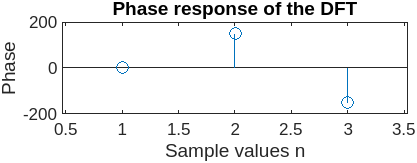
\includegraphics[width=0.8\textwidth]{phaseDFT.png}
    \caption{DFT phase response}
    \label{fig:dft_result}
\end{figure}
\section{ Inverse Discrete Fourier Transform (IDFT)}
 The Fourier transform maps a time-domain signal into the frequency domain,
 preserving all information. The inverse Fourier transform converts the signal
 back to the time domain. The Discrete Fourier Transform (DFT) converts a
 discrete-time signal into its frequency domain representation. Given a sequence x(n) of length N, its DFT is given by:
 \begin{equation}
    x(n) = \frac{1}{N} \sum_{k=0}^{N-1} X(k) e^{j \frac{2\pi}{N} kn}, \quad n = 0,1,\dots,N-1
\end{equation}
\subsection{MATLAB Code  for IDFT}
\begin{minted}[frame=single,fontsize=\small]{matlab} 
clc;
 clear all;
 close all;
 a=input('Enter the sequence :');
 N=length(a);
 disp('The length of the sequence is:');N
 for n=1:N
 y(n)=0;
 for k=1:N
 y(n)=y(n)+a(k)*exp((2*pi*j*(k-1)*(n-1))/N);
 end;
 end;
 n=1:N
 y1=1/N*y(n);
 disp('The result is:');y1
 figure(1);
 stem(n,y1);
 xlabel('Sample values n');
 ylabel('Amplitude');
 title(Magnitude response of the IDFT');
\end{minted}
\subsection{Results for IDFT}
In this implementation, the input sequence is transformed back into the time domain using the IDFT formula. The computed values are then normalized by \( 1/N \) to obtain the original sequence. The resulting time-domain samples are visualized using a stem plot, which highlights the discrete nature of the reconstructed signal.
\textbf{Key Takeaway:} The IDFT accurately recovers the original time-domain signal from its frequency components, demonstrating the fundamental concept of spectral decomposition and reconstruction in digital signal processing.
\begin{figure}[h]
    \centering
    \includegraphics[width=0.5\textwidth]{IDFT (2).png}
    \caption{IDFT Magnitude response}
    \label{fig:dft_result}
\end{figure}
\section{Finding the FFT of Different Signals}
 The IDFT reconstructs a sequence from its DFT.The inverse DFT (IDFT) reconstructs the original sequence from its frequency domain representation
 
\subsection{Program Description}
In this program, we use the command FFT to compute the impulse response. In the process of finding the FFT, the length of the FFT is taken as $N$. The FFT consists of two parts: 
\begin{itemize}
    \item 	extbf{Magnitude Plot:} The absolute value of magnitude versus the samples.
    \item 	extbf{Phase Plot:} The phase angle versus the samples.
\end{itemize}
\begin{minted}[frame=single,fontsize=\small]{matlab} 
clc;
 clear all;
 close all;
 t=-2:1:2;
 y=[zeros(1,2) 1 zeros(1,2)];
 subplot (3,1,1);
 stem(t,y);
 grid;
 4
title ('Impulse Response');
 xlabel ('Time');
 ylabel ('Amplitude');
 N=input('Enter the length of the FFT sequence: ');
 xk=fft(y,N);
 magxk=abs(xk);
 angxk=angle(xk);
 k=0:N-1;
 subplot(3,1,2);
 stem(k,magxk);
 xlabel('k');
 ylabel('|x(k)|');
 subplot(3,1,3);
 stem(k,angxk);
 xlabel('k');
 ylabel('arg(x(k))');
\end{minted}
\subsection{Results for FFT}
The Fast Fourier Transform (FFT) is an efficient algorithm for computing the Discrete Fourier Transform (DFT) of a sequence. In this implementation, we compute the FFT of an impulse response, which is a fundamental signal in signal processing. The impulse response is represented as a discrete-time signal, where a single nonzero value occurs at a specific position while all other values remain zero.

The program first defines the impulse response and plots it in the time domain. The FFT of this sequence is then computed over a length \( N \), transforming the signal into the frequency domain. The results are visualized through two key plots: 

Magnitude Spectrum: The absolute values of the FFT coefficients, representing the strength of different frequency components in the signal.
- Phase Spectrum: The phase angles of the FFT coefficients, indicating the phase shift of each frequency component.

By analyzing these plots, we can observe how the impulse response is distributed across different frequencies. Since an impulse in the time domain contains all frequency components equally, its FFT exhibits a flat magnitude response, confirming its role as a fundamental building block in signal analysis.

\begin{figure}[h]
    \centering
    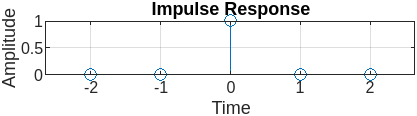
\includegraphics[width=0.8\textwidth]{FFT.png}
    \caption{FFT Impulse Response in MATLAB}
    \label{fig:dft_result}
\end{figure}
\begin{figure}[h]
    \centering
    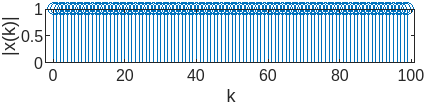
\includegraphics[width=0.8\textwidth]{FFTangle.png}
    \caption{FFT phase representation in MATLAB}
    \label{fig:dft_result}
\end{figure}
\begin{figure}[h]
    \centering
    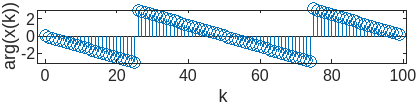
\includegraphics[width=0.8\textwidth]{FFTphase.png}
    \caption{FFT angle Representation in MATLAB}
    \label{fig:dft_result}
\end{figure}
\section{Lab Task}
\subsection{Impulse Response and DFT Computation}
\subsubsection{MATLAB Code for DFT}
Sequence we used is  x = [1,2,3,4], h = [4,3,2,1].

\begin{minted}[frame=single,fontsize=\small]{matlab} 
clc;
 clear all;
 close all;
 a=input('Enter the sequence :');
 N=length(a);
 disp('he length of the sequence is:');N
 for k=1:N
 y(k)=0;
 for i=1:N
 y(k)=y(k)+a(i)*exp((-2*pi*j/N)*((i-1)*(k-1)));
 end;
 end;
 k=1:N
 disp('The result is:');y
 figure(1);
 subplot(211);
 stem(k,abs(y(k)));
 xlabel('Sample values n');
 ylabel('Amplitude');
 title('Magnitude response of the DFT');
 subplot(212);
 stem(angle(y(k))*180/pi);
 xlabel('Sample values n');
 ylabel('Phase');
 title('phase response of the DFT');
\end{minted}

\subsubsection{Results for DFT}
The Discrete Fourier Transform (DFT) of a given sequence is computed using the formula:

\[
Y(k) = \sum_{i=0}^{N-1} a(i) e^{-j(2\pi/N) (i-1)(k-1)}
\]

where \( a(i) \) represents the input sequence, and \( Y(k) \) is the transformed sequence in the frequency domain.

The magnitude response plot shows how the energy of the signal is distributed across different frequency components. Peaks in the magnitude spectrum indicate dominant frequency components present in the input sequence.

The phase response plot illustrates the phase shift associated with each frequency component. The phase spectrum is crucial in signal reconstruction, as it determines the alignment of sinusoidal components in the time domain.

\textbf{Key Takeaway:} The DFT decomposes a time-domain signal into its constituent frequency components, providing insight into the frequency content and phase characteristics of the sequence.
\begin{figure}[h]
    \centering
    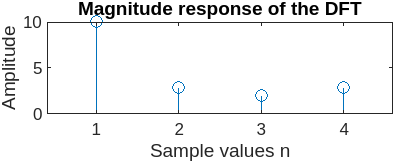
\includegraphics[width=0.8\textwidth]{taskm_dft_result.png}
    \caption{Impulse Response DFT Magnitude in MATLAB}
    \label{fig:impulse_fft_result}
\end{figure}
\begin{figure}[h]
    \centering
    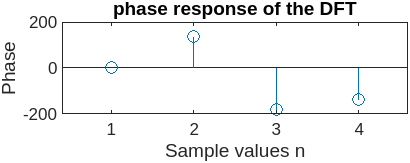
\includegraphics[width=0.8\textwidth]{taskp_dft_result.png}
    \caption{Impulse Response DFT Phase in MATLAB}
    \label{fig:impulse_fft_result}
\end{figure}
\subsection{Impulse Response and FFT Computation}

\subsubsection{MATLAB Code for step sequence for FFT}
\begin{minted}[frame=single,fontsize=\small]{matlab}
clear; close all;

N = 8; % Length of sequence
n = 0:N-1;

% Step Sequence
u = ones(1, N);
U = fft(u);

% Plot Step Sequence and FFT
figure;

subplot(3,1,1);
stem(n, u, 'filled'); title('Step Sequence');
xlabel('n'); ylabel('Amplitude');

subplot(3,1,2);
stem(n, abs(U), 'filled'); title('Magnitude of FFT (Step)');
xlabel('Frequency index'); ylabel('|U(k)|');

subplot(3,1,3);
stem(n, angle(U), 'filled'); title('Phase of FFT (Step)');
xlabel('Frequency index'); ylabel('Phase(U(k))');

\end{minted}

\subsubsection{Results for step sequence}
The step sequence is a constant signal, meaning it has a flat amplitude of 1 for all values of \( n \). It appears as a horizontal line at 1 in the stem plot.

The FFT of a step sequence results in a DC-dominated frequency spectrum. The first frequency component (DC component, \( k=0 \)) has the highest magnitude because the sequence has a constant average value. The remaining components decay quickly.

The phase is mostly zero, except for some frequency components which may have a small phase shift due to numerical approximations in FFT calculations.

\textbf{Key Takeaway:} The step function contains mainly low-frequency components because it does not change rapidly over time.
\begin{figure}[h]
    \centering
    \includegraphics[width=0.8\textwidth,frame, clip]{Screenshot 2025-02-25 221729.png}
    \caption{Magnitude of Step Sequence FFT for step function}
    \label{fig:impulse_fft_result}
\end{figure}


\subsubsection{MATLAB Code for ramp sequence for FFT}

\begin{minted}[frame=single,fontsize=\small]{matlab}
clc; clear; close all;

N = 8; % Length of sequence
n = 0:N-1;

% Ramp Sequence
r = 0:N-1;
R = fft(r);

% Plot Ramp Sequence and FFT
figure;

subplot(3,1,1);
stem(n, r, 'filled'); title('Ramp Sequence');
xlabel('n'); ylabel('Amplitude');

subplot(3,1,2);
stem(n, abs(R), 'filled'); title('Magnitude of FFT (Ramp)');
xlabel('Frequency index'); ylabel('|R(k)|');

subplot(3,1,3);
stem(n, angle(R), 'filled'); title('Phase of FFT (Ramp)');
xlabel('Frequency index'); ylabel('Phase(R(k))');

\end{minted}
\subsubsection{Results for ramp function}
The ramp sequence is a linearly increasing function: \( r[n] = n \). This means higher values appear as \( n \) increases.

The magnitude of the FFT for a ramp function decreases gradually but does not vanish at higher frequencies. Unlike the step sequence, which has strong DC components, the ramp sequence contains higher frequency components due to its increasing nature.

The phase varies significantly across frequencies. The ramp sequence has a non-trivial phase pattern because it contains multiple frequency components.

\textbf{Key Takeaway:} A ramp function has stronger high-frequency components than a step function, making its magnitude spectrum more spread out.

\begin{figure}[h]
    \centering
    \includegraphics[width=0.8\textwidth,frame, clip]{Screenshot 2025-02-25 222018.png}
    \caption{Amplitude,Magnitude and Phase of ramp function}
    \label{fig:impulse_fft_result}
\end{figure}

\subsubsection{MATLAB Code for exponential function using FFT}
\begin{minted}[frame=single,fontsize=\small]{matlab}
clc; clear; close all;

N = 8; % Length of sequence
n = 0:N-1;
a = 0.2;

% Exponential Sequence
exp_seq = exp(a*n);
Exp_FFT = fft(exp_seq);

% Plot Exponential Sequence and FFT
figure;

subplot(3,1,1);
stem(n, exp_seq, 'filled'); 
title('Exponential Sequence');
xlabel('n'); ylabel('Amplitude');

subplot(3,1,2);
stem(n, abs(Exp_FFT), 'filled'); 
title('Magnitude of FFT (Exponential)');
xlabel('Frequency index'); ylabel('|X(k)|');

subplot(3,1,3);
stem(n, angle(Exp_FFT), 'filled'); 
title('Phase of FFT (Exponential)');
xlabel('Frequency index'); ylabel('Phase(X(k))');


\end{minted}
\subsubsection{Results for exponential function}
The exponential sequence grows exponentially as \( x[n] = e^{0.2n} \). Since \( e^{0.2n} \) increases rapidly, the values grow large as \( n \) increases.

The FFT of an exponential function shows a peak at a specific frequency. This is because the exponential function can be represented as a sum of sinusoidal components at a particular frequency. The magnitude plot has one strong peak, showing that the exponential sequence is concentrated around one frequency.

The phase varies smoothly and shows a clear frequency dependency. The pattern of the phase shift tells us how the signal’s frequency content is distributed.

\textbf{Key Takeaway:} The exponential sequence behaves like a sinusoidal function at a specific frequency, leading to a localized frequency peak in its magnitude spectrum.
\begin{figure}[h]
    \centering
    \includegraphics[width=0.5\textwidth,frame, clip]{Screenshot 2025-02-25 222311.png}
    \caption{Amplitude, Magnitude and Phase of exponential function}
    \label{fig:impulse_fft_result}
\end{figure}

\end{document}
